{\em Heyawake} ist ein japanisches Rätsel, welches auf einem $n\times m$-Feld
gespielt wird. Das Spielfeld ist durch dickere Linien unterteilt in grössere rechteckige Gebiete, die {\it Zimmer} genannt werden. 
Ziel des Spieles ist, einzelne Felder schwarz einzufärben, so dass die
folgenden Regeln erfüllt sind:
\begin{enumerate}
\item
Schwarze Quadrate grenzen niemals über eine Kante aneinander.
\item
Alle weissen Quadrate hängen über Kanten zusammen.
\item
Die Zahlen geben an, wie viele schwarze Quadrate in einem Zimmer vorkommen.
\item
Ein Zimmer ohne Zahl kann beliebig viele schwarze Quadrate enthalten
(solange die anderen Regeln erfüllt sind).
\item
Eine gerade (horizontale oder vertikale) Linie aus zusammenhängenden
weissen Quadraten kann sich höchstens über zwei Zimmer erstrecken.
\end{enumerate}
Das folgende Beispiel zeigt Aufgabe und Lösung:
\begin{center}
\includeagraphics[width=0.35\hsize]{solution-big.png}
\qquad
\includeagraphics[width=0.35\hsize]{example-big.png}
\end{center}

Kann eine nichtdeterministische Maschine in polynomieller Zeit entscheiden,
ob ein Heyawake-Rätsel eine Lösung hat?

\thema{NP}
\thema{polynomieller Verifizierer}

\begin{loesung}
Das Problem ist sicher entscheidbar, man kann alle $2^{nm}$ Einfärbungen
daraufhin überprüfen, ob die Regeln eingehalten werden.
Dafür ist allerdings exponentielle Zeit notwendig.

Eine nichtdeterministische Maschine kann die Entscheidungsfrage genau
dann in polynomieller Zeit beantworten, wenn es einen polynomiellen
Verifizierer gibt.
Als Lösungszertifikat $c$ fordern wir die Belegung der schwarzen Felder.
Der Verfikationsalgorithmus muss die Regeln 1--5 überprüfen, und braucht
dafür Zeit wie folgt
\begin{center}
\begin{tabular}{r|l|>{$}c<{$}}
Regel&Arbeit&\text{Aufwand}\\
\hline
1.&Für jedes schwarze Feld 4 Nachbarn überprüfen&O(nm)\\
2.&Zusammenhang überprüfen&O(n^2m^2)\\
3.&Für jede Zahl die Anzahl schwarzer Felder im Zimmer prüfen&O(nm)\\
4.&automatisch erfüllt nach 3.&0\\
5.&Für jedes weisse Feld, überprüfe Zeilenlänge&O(nm(n+m))\\
\hline
&$c$ ist Lösung des Heyawake-Rätsels&O(n^2m^2)
\end{tabular}
\end{center}
Nur die Überprüfung des Zusammenhangs ist etwas anspruchsvoller.
Man kann dazu einen Einfärbe-Algorithmus verwenden:
\begin{enumerate}
\item Markiere das erste weisse Feld {\color{red}rot}.
\item Für jedes {\color{red}rot} markierte Feld markiere 
alle noch nicht {\color{red}rot} markierten weissen Nachbarfelder ebenfalls
{\color{red}rot}.
\item Wiederhole Schritt 2, bis sich in einem Durchgang keine weiteren
Felder einfärben liessen.
\end{enumerate}
Wenn am Ende dieses Algorithmus weisse Felder übrig bleiben, ist die
in Regel~2 formulierte Bedinung nicht erfüllt.
Der Färbealgorithmus besucht in jedem Durchgang jedes Feld höchstens einmal,
braucht also für einen Durchgang die Zeit $O(nm)$.
Im schlimmsten Fall ändert in jedem Durchgang nur ein einziges Feld seine
Farbe, es braucht also $O(nm)$ Durchgänge.
Der gesamte Zeitaufwand für die Überprüfung des Zusammenhangs
ist daher $O(n^2m^2)$.

Die Überprüfung der Regel~5 muss in jedem der $nm$-Felder höchstens $n$
vertikale und $m$ vertikale Felder überprüfen, dafür ist Zeit
$O(nm(n+m))$ nötig.

Damit ist gezeigt, dass es einen polynomiellen Verifizierer gibt, und
es folgt, dass eine nichtdeterministische Maschine ein Heyawake-Rätsel
in polynomieller Zeit lösen kann.
\end{loesung}

\begin{diskussion}
Der schwierigste Schritt im Verifikationsalgorithmus ist die Überprüfung
des Zusammenhangs der weissen Felder.
Es reicht leider nicht, nur zu prüfen, ob jedes weisse Feld auch einen
weissen Nachbarn hat.
Damit kann man nur weisse Felder finden, die vollständig von schwarzen
Feldern eingeschlossen sind.
Das folgende Feld erfüllt die Bedingung, trotzdem sind die weissen
Felder nicht zusammenhängend:
\begin{center}
\def\h{1}
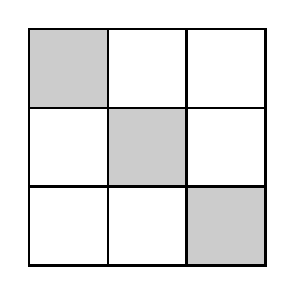
\begin{tikzpicture}
\fill[color=gray!40] (0,0) rectangle (\h,-\h);
\fill[color=gray!40] (\h,-\h) rectangle ++(\h,-\h);
\fill[color=gray!40] ({2*\h},{-2*\h}) rectangle ++(\h,-\h);
\draw[line width=0.8pt] (\h,0) -- ++(0,{-3*\h});
\draw[line width=0.8pt] ({2*\h},0) -- ++(0,{-3*\h});
\draw[line width=0.8pt] (0,-\h) -- ++({3*\h},0);
\draw[line width=0.8pt] (0,{-2*\h}) -- ++({3*\h},0);
\draw[line width=1pt] (0,0) rectangle ({3*\h},{-3*\h});
\end{tikzpicture}
\end{center}

Man könnte versucht sein, den Färbealgorithmus zur Feststellung des
Zusammenhangs rekursiv zu formulieren, dabei trifft man jedoch auf ein
Dilemma.
Wenn man von jedem Feld rekursiv alle Nachbarn untersucht, dann besucht
man jedes Feld mehrmals, insbesondere wächst die Zahl der Feldbesuche
exponentiell, man kann so also keinen polynomiellen Algorithmus bekommen.
Wenn man nur die weissen Nachbarfelder besucht, dann findet man nicht
alle Felder, denn im Schritt zwei werden ja Felder rot eingefärbt, ohne 
dass man prüft, ob sie weisse Nachbarn haben.
Diese weissen Nachbarn wird man dann möglicherweise nicht mehr einfärben
können.
Die iterative Formulierung vermeidet diese Schwierigkeit.

Die Frage, ob ein Heyawake-Rätsel eine Lösung hat, ist NP-vollständig:
Markus Holzer und Oliver Ruepp, {\it The Troubles of Interior Design--A
Complexity Analysis of the Game Heyawake}, Proceedings,
4th International Conference on Fun with Algorithms, LNCS 4475, Springer,
Berlin/Heidelberg, 2007, pp.~198-212.
\end{diskussion}

\begin{bewertung}
Verwendung eines Verifizierers ({\bf V}) 1 Punkt,
Lösungszertifikat spezifiziert ({\bf L}) 1 Punkt,
Anzahl schwarze Felder überprüft ({\bf S}) 1 Punkt,
Zusammenhang überprüft ({\bf Z}) 1 Punkt,
Nachbarschaft und Zeilenlänge ({\bf N}) 1 Punkt,
Zeitaufwand ist polynomiell ({\bf P}) 1 Punkt.
\end{bewertung}
